\documentclass[12pt,a4paper]{article}

% ─── Page Layout ───────────────────────────────────────────────────────────────
\usepackage[a4paper, margin=0.8in, headheight=14pt]{geometry}

% ─── Fonts (XeLaTeX) ───────────────────────────────────────────────────────────
\usepackage{fontspec}
\usepackage{unicode-math}
\setmainfont{TeX Gyre Pagella}
\setmonofont[Scale=0.88]{TeX Gyre Cursor}
\setmathfont{Latin Modern Math}

% ─── Packages ──────────────────────────────────────────────────────────────────
\usepackage{xcolor}
\usepackage{colortbl}
\usepackage{titlesec}
\usepackage{enumitem}
\usepackage{tabularx}
\usepackage{booktabs}
\usepackage{array}
\usepackage{amsmath}
\usepackage{tikz}
\usetikzlibrary{shapes.geometric, arrows.meta, positioning, calc, fit, decorations.pathreplacing}
\usepackage{tcolorbox}
\tcbuselibrary{skins, breakable}
\usepackage{hyperref}
\usepackage{fancyhdr}
\usepackage{graphicx}
\usepackage{microtype}
\hyphenpenalty=10000
\exhyphenpenalty=10000
\sloppy
\usepackage{caption}
\usepackage{setspace}
\usepackage{multirow}
\usepackage{tocloft}

% ─── Q&A helper ────────────────────────────────────────────────────────────────
\newcommand{\Q}[1]{\textbf{#1}\par\noindent\ignorespaces}

% ─── Colour Palette ────────────────────────────────────────────────────────────
\definecolor{myred}{RGB}{196,30,58}
\definecolor{mydark}{RGB}{30,30,50}
\definecolor{mygreen}{RGB}{14,120,80}
\definecolor{myteal}{RGB}{0,130,140}
\definecolor{myamber}{RGB}{180,100,0}
\definecolor{mypurple}{RGB}{100,30,160}
\definecolor{mygray}{RGB}{246,247,249}
\definecolor{mgframe}{RGB}{180,185,200}
\definecolor{watermark}{RGB}{145,150,170}
\definecolor{hdrred}{RGB}{250,232,235}
\definecolor{hdrgreen}{RGB}{220,244,233}
\definecolor{hdrteal}{RGB}{220,242,244}
\definecolor{hdramber}{RGB}{253,242,215}
\definecolor{hdrpurple}{RGB}{238,228,255}
\definecolor{hdrgray}{RGB}{238,240,245}
\definecolor{rowalt}{RGB}{250,251,253}

% ─── Section Formatting ────────────────────────────────────────────────────────
\titleformat{\section}
  {\large\bfseries\color{myred}}{\thesection.}{0.5em}{}
  [\vspace{1pt}{\color{myred}\rule{\linewidth}{0.8pt}}]
\titleformat{\subsection}
  {\normalsize\bfseries\color{myteal}}{\thesubsection}{0.5em}{}
\titlespacing*{\section}{0pt}{18pt}{7pt}
\titlespacing*{\subsection}{0pt}{11pt}{4pt}

% ─── Paragraph ─────────────────────────────────────────────────────────────────
\setlength{\parindent}{0pt}
\setlength{\parskip}{4pt}

% ─── TOC Styling ───────────────────────────────────────────────────────────────
\renewcommand{\cfttoctitlefont}{\large\bfseries\color{myred}}
\renewcommand{\cftaftertoctitle}{\par\noindent{\color{myred}\rule{\linewidth}{0.8pt}}}
\setlength{\cftbeforetoctitleskip}{0pt}
\setlength{\cftaftertoctitleskip}{6pt}
\renewcommand{\cftsecfont}{\normalsize\bfseries\color{mydark}}
\renewcommand{\cftsecpagefont}{\normalsize\bfseries\color{mydark}}
\renewcommand{\cftsecleader}{\cftdotfill{\cftdotsep}}
\setlength{\cftbeforesecskip}{7pt}
\renewcommand{\cftsubsecfont}{\small\color{mydark}}
\renewcommand{\cftsubsecpagefont}{\small\color{mydark}}
\setlength{\cftbeforesubsecskip}{3pt}
\setlength{\cftsubsecindent}{1.4em}

% ─── Table helpers ─────────────────────────────────────────────────────────────
\renewcommand{\arraystretch}{1.45}
\setlength{\tabcolsep}{6pt}
\arrayrulecolor{mydark}
\newcolumntype{B}[1]{>{\small\bfseries\raggedright\arraybackslash}m{#1}}
\newcolumntype{Y}{>{\small\raggedright\arraybackslash}X}
\renewcommand{\tabularxcolumn}[1]{m{#1}}

% ─── Header / Footer ───────────────────────────────────────────────────────────
\pagestyle{fancy}
\fancyhf{}
\fancyhead[L]{\small\color{myred}\textbf{PE-EC703B}\;\color{mydark}--- Wireless Sensor Networks}
\fancyhead[R]{\small\color{myteal}\textbf{Module 1 Notes}}
\fancyfoot[C]{\small\color{mydark}\thepage}
\fancyfoot[R]{\small\color{watermark}\textit{\copyright\ Biraj}}
\renewcommand{\headrulewidth}{0.5pt}
\renewcommand{\footrulewidth}{0.3pt}

% ─── Hyperref ──────────────────────────────────────────────────────────────────
\hypersetup{
  colorlinks=true, linkcolor=myteal, urlcolor=myteal,
  pdfauthor={Biraj Sarkar},
  pdftitle={PE-EC703B --- Module 1 Notes}
}

% ─── tcolorbox styles ──────────────────────────────────────────────────────────
\tcbset{
  tikzbox/.style={
    colback=mygray, colframe=mgframe, boxrule=0.6pt, arc=4pt,
    left=8pt, right=8pt, top=6pt, bottom=6pt,
    colbacktitle=mgframe, coltitle=mydark,
    fonttitle=\small\bfseries
  },
  defbox/.style={
    colback=hdrgreen, colframe=mygreen, boxrule=0.8pt, arc=4pt,
    left=9pt, right=9pt, top=6pt, bottom=6pt,
    colbacktitle=mygreen, coltitle=white,
    fonttitle=\small\bfseries
  },
  formulabox/.style={
    colback=hdrteal, colframe=myteal, boxrule=0.8pt, arc=4pt,
    left=9pt, right=9pt, top=7pt, bottom=7pt,
    colbacktitle=myteal, coltitle=white,
    fonttitle=\small\bfseries
  },
  examplebox/.style={
    colback=hdramber, colframe=myamber, boxrule=0.8pt, arc=4pt,
    left=9pt, right=9pt, top=6pt, bottom=6pt,
    colbacktitle=myamber, coltitle=white,
    fonttitle=\small\bfseries
  },
  masonbox/.style={
    colback=hdrpurple, colframe=mypurple, boxrule=0.8pt, arc=4pt,
    left=9pt, right=9pt, top=6pt, bottom=6pt,
    colbacktitle=mypurple, coltitle=white,
    fonttitle=\small\bfseries
  },
  exambox/.style={
    colback=hdrpurple, colframe=mypurple, boxrule=1pt, arc=5pt,
    left=10pt, right=10pt, top=8pt, bottom=8pt,
    colbacktitle=mypurple, coltitle=white,
    fonttitle=\bfseries,
    breakable, title after break={\textbf{Frequently Asked / Viva Questions (contd.)}}}
}
% Make all boxes breakable across pages
\tcbset{breakable}

% ─── TikZ styles ───────────────────────────────────────────────────────────────
\tikzset{
  block/.style={rectangle, draw=myteal, fill=hdrteal,
    text width=2.4cm, align=center, minimum height=0.95cm,
    font=\small, rounded corners=3pt, line width=0.7pt},
  redblock/.style={rectangle, draw=myred, fill=hdrred,
    text width=2.4cm, align=center, minimum height=0.95cm,
    font=\small, rounded corners=3pt, line width=0.7pt},
  netnode/.style={rectangle, draw=myteal, fill=hdrteal,
    text width=1.5cm, align=center, minimum height=0.8cm,
    font=\small, rounded corners=3pt, line width=0.7pt},
  sumjunc/.style={circle, draw=myamber, fill=hdramber,
    minimum size=0.62cm, font=\small, line width=0.8pt},
  snode/.style={circle, draw=mypurple, fill=hdrpurple,
    minimum size=0.55cm, font=\footnotesize, line width=0.7pt},
  arrow/.style={-Stealth, thick, color=mydark},
  redarrow/.style={-Stealth, thick, color=myred},
  line/.style={thick, color=mydark}
}

% ═══════════════════════════════════════════════════════════════════════════════
\begin{document}
% ═══════════════════════════════════════════════════════════════════════════════

\begin{center}
  {\LARGE\bfseries\color{myred} PE-EC703B --- Wireless Sensor Networks}\\[5pt]
  {\normalsize\color{mydark} Semester VII \quad$\bullet$\quad 3L:0T:0P \quad$\bullet$\quad 3 Credits}\\[3pt]
  {\normalsize\color{myteal}\textbf{Module 1 Exam Notes: Introduction to Wireless Sensor Networks}}\\[3pt]
  {\small\color{mydark} CGEC \;$|$\; B.Tech ECE (2023--27) \;$|$\; \textit{Biraj Sarkar}}
\end{center}
\vspace{2pt}
\noindent{\color{myred}\rule{\linewidth}{1.5pt}}
\vspace{2pt}

\hypersetup{linkcolor=mydark}
\tableofcontents
\hypersetup{linkcolor=myteal}
\newpage

% ===============================================================================
\section{What is a Wireless Sensor Network?}
% ===============================================================================

A Wireless Sensor Network (WSN) is a distributed network of small, low-power sensor nodes that are spatially deployed to monitor physical or environmental conditions and cooperatively communicate data to a central point (sink or base station).

\begin{tcolorbox}[defbox, title={\textbf{Wireless Sensor Network (WSN) --- Definition}}]
A \textbf{Wireless Sensor Network} is a self-organizing collection of spatially distributed, resource-constrained sensor nodes that sense physical parameters (temperature, pressure, motion, light, etc.) and transmit collected data wirelessly, usually through multi-hop communication, to a \textbf{sink node} or \textbf{base station} for processing and action.
\end{tcolorbox}

A WSN consists of:
\begin{itemize}[leftmargin=*, itemsep=3pt]
  \item \textbf{Sensor nodes (motes):} Battery-powered miniature devices with sensing, processing, and wireless communication capability.
  \item \textbf{Sink node (base station):} Aggregates all data from sensor nodes and forwards to an external network or user.
  \item \textbf{Task manager node:} Issues tasks (queries) into the network and receives aggregated results.
  \item \textbf{Communication medium:} Wireless radio (IEEE 802.15.4, ZigBee, Bluetooth LE).
\end{itemize}

\begin{tcolorbox}[tikzbox, title={WSN Architecture --- Sensing Field to User}]
\centering
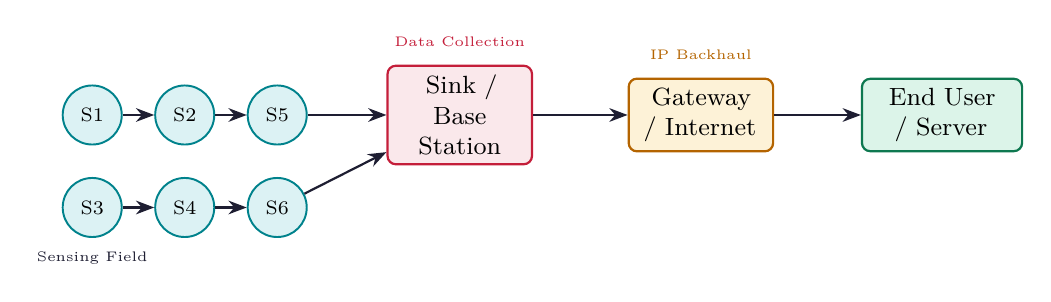
\begin{tikzpicture}[node distance=0.5cm and 1.1cm,
  wsnode/.style={circle, draw=myteal, fill=hdrteal, minimum size=0.75cm, font=\scriptsize, align=center, line width=0.7pt},
  sinknode/.style={rectangle, draw=myred, fill=hdrred, text width=1.6cm, align=center, minimum height=0.85cm, font=\small, rounded corners=3pt, line width=0.8pt},
  gwnode/.style={rectangle, draw=myamber, fill=hdramber, text width=1.6cm, align=center, minimum height=0.85cm, font=\small, rounded corners=3pt, line width=0.8pt},
  usernode/.style={rectangle, draw=mygreen, fill=hdrgreen, text width=1.8cm, align=center, minimum height=0.85cm, font=\small, rounded corners=3pt, line width=0.8pt}]

  % Sensor nodes
  \node[wsnode] (n1) {S1};
  \node[wsnode, right=0.4cm of n1] (n2) {S2};
  \node[wsnode, below=0.4cm of n1] (n3) {S3};
  \node[wsnode, right=0.4cm of n3] (n4) {S4};
  \node[wsnode, right=0.4cm of n2] (n5) {S5};
  \node[wsnode, right=0.4cm of n4] (n6) {S6};

  % Sink
  \node[sinknode, right=1.0cm of n5] (sink) {Sink / Base Station};

  % Gateway
  \node[gwnode, right=1.2cm of sink] (gw) {Gateway / Internet};

  % User
  \node[usernode, right=1.1cm of gw] (usr) {End User / Server};

  % Arrows: sensor to sensor (multi-hop)
  \draw[arrow] (n1) -- (n2);
  \draw[arrow] (n3) -- (n4);
  \draw[arrow] (n2) -- (n5);
  \draw[arrow] (n4) -- (n6);
  \draw[arrow] (n5) -- (sink);
  \draw[arrow] (n6) -- (sink);
  \draw[arrow] (sink) -- (gw);
  \draw[arrow] (gw) -- (usr);

  % Labels
  \node[font=\tiny, color=mydark, below=0.05cm of n3] {Sensing Field};
  \node[font=\tiny, color=myred, above=0.1cm of sink] {Data Collection};
  \node[font=\tiny, color=myamber, above=0.1cm of gw] {IP Backhaul};
\end{tikzpicture}
\end{tcolorbox}

% ===============================================================================
\section{Unique Constraints and Challenges in WSN}
% ===============================================================================

WSNs operate under severe resource limitations that do not apply to traditional networks. These constraints fundamentally drive the design of every protocol and algorithm in WSN.

\subsection{Unique Constraints}

\begin{tcolorbox}[formulabox, title={\textbf{Key Constraints of WSN}}]
\begin{enumerate}[leftmargin=*, itemsep=4pt]
  \item \textbf{Energy constraint:} Sensor nodes are battery-powered with limited energy. Replacing batteries is often impractical (nodes deployed in remote or harsh environments). Energy governs node lifetime and hence network lifetime.
  \item \textbf{Computation constraint:} Nodes have very limited processing power (e.g., 8-bit or 16-bit microcontrollers at 4--16 MHz). Complex algorithms cannot run on-node.
  \item \textbf{Memory constraint:} Typically only 4--10 KB RAM and 48--256 KB flash. Large routing tables or data buffers are infeasible.
  \item \textbf{Communication constraint:} Short-range radio (10--100 m), low bandwidth (20--250 kbps), high bit-error rates, and half-duplex operation.
  \item \textbf{Physical size constraint:} Nodes must be very small (mote form factor); this restricts antenna size, battery capacity, and sensor quality.
  \item \textbf{Cost constraint:} Mass deployment requires nodes to be cheap (Rs.~100--2000 per node). This limits hardware quality.
\end{enumerate}
\end{tcolorbox}

\subsection{Challenges}

\begin{itemize}[leftmargin=*, itemsep=3pt]
  \item \textbf{Scalability:} Networks may contain hundreds to thousands of nodes. Protocols must scale without central control.
  \item \textbf{Fault tolerance:} Nodes fail due to battery depletion or physical damage. The network must self-heal and reroute.
  \item \textbf{Dynamic topology:} Nodes may join, leave, or move; links break frequently. Routing must adapt dynamically.
  \item \textbf{Data-centric communication:} Unlike address-centric IP networks, WSN queries are about \emph{what} data (e.g., ``temperature $> 50$°C''), not \emph{where} a node is.
  \item \textbf{Localization:} Knowing the geographic position of a node is essential for many applications but GPS is expensive and power-hungry.
  \item \textbf{Synchronization:} Nodes need time-synchronized sleep/wake cycles; clocks drift over time.
  \item \textbf{Security:} Nodes operate in hostile environments; attackers can eavesdrop, inject, or jam communications.
  \item \textbf{QoS:} Latency, reliability, and data freshness requirements vary by application.
\end{itemize}

% ===============================================================================
\section{Advantages of Sensor Networks}
% ===============================================================================

\begin{tcolorbox}[examplebox, title={\textbf{Why Use WSNs? --- Key Advantages}}]
\begin{itemize}[leftmargin=*, itemsep=4pt]
  \item \textbf{Infrastructure-free deployment:} No cables or fixed infrastructure needed. Nodes can be air-dropped or scattered over terrain.
  \item \textbf{Dense spatial coverage:} Hundreds of nodes provide granular, distributed sensing impossible with a single instrument.
  \item \textbf{Real-time monitoring:} Continuous data collection and event detection without human presence.
  \item \textbf{Self-organizing:} Nodes autonomously form a network, discover neighbors, and elect cluster heads.
  \item \textbf{Fault tolerance:} Redundant nodes maintain coverage even when individual nodes fail.
  \item \textbf{Cost-effective:} Mass production makes per-node cost very low; no installation labor needed.
  \item \textbf{Accessibility:} Can operate in hazardous, remote, or physically inaccessible environments (volcanoes, battlefields, pipelines).
  \item \textbf{Long-term monitoring:} With proper sleep scheduling, networks can last months to years.
\end{itemize}
\end{tcolorbox}

% ===============================================================================
\section{Applications of Sensor Networks}
% ===============================================================================

WSNs are used across virtually every domain requiring unattended, distributed data collection.

\par\noindent
{\renewcommand{\arraystretch}{1.5}%
\begin{tabularx}{\linewidth}{|B{3.0cm}|Y|Y|}
\hline
\textbf{Domain} & \textbf{Application} & \textbf{Parameters Sensed} \\
\hline
\textbf{Military} & Battlefield surveillance, intrusion detection, target tracking & Motion, acoustic, seismic \\
\hline
\textbf{Environment} & Forest fire detection, flood monitoring, wildlife tracking & Temperature, humidity, CO$_2$, water level \\
\hline
\textbf{Health / Medical} & Patient monitoring, assisted living, drug delivery & Heart rate, blood pressure, glucose, posture \\
\hline
\textbf{Industrial} & Machine condition monitoring, pipeline leak detection, factory automation & Vibration, pressure, flow, temperature \\
\hline
\textbf{Agriculture} & Precision farming, soil moisture, irrigation control & Soil pH, moisture, light, temperature \\
\hline
\textbf{Smart Home} & Appliance control, security, energy management & Light, motion, temperature, CO levels \\
\hline
\textbf{Infrastructure} & Structural health monitoring of bridges, buildings & Strain, vibration, tilt, displacement \\
\hline
\textbf{Transportation} & Vehicle detection, traffic management, parking & Magnetic, acoustic, optical \\
\hline
\end{tabularx}}

% ===============================================================================
\section{Types of Wireless Sensor Networks}
% ===============================================================================

WSNs are classified based on deployment medium, node mobility, and communication model.

\subsection{Based on Deployment Medium}

\par\noindent
{\renewcommand{\arraystretch}{1.5}%
\begin{tabularx}{\linewidth}{|B{3.2cm}|Y|Y|}
\hline
\textbf{Type} & \textbf{Description} & \textbf{Applications} \\
\hline
\textbf{Terrestrial WSN} & Nodes deployed on land; communicate via ground-level radio; most common type & Environmental monitoring, agriculture, smart cities \\
\hline
\textbf{Underground WSN} & Nodes buried in soil; signals travel through earth; high attenuation; expensive & Pipeline monitoring, precision agriculture \\
\hline
\textbf{Underwater WSN} & Nodes deployed in water; use acoustic communication (RF attenuates rapidly in water); low bandwidth, high delay & Oceanographic data collection, pollution detection \\
\hline
\textbf{Multimedia WSN} & Nodes equipped with cameras, microphones; high data rate; large bandwidth demand & Surveillance, traffic monitoring \\
\hline
\textbf{Mobile WSN} & Nodes can move (mobile robots, vehicles); topology changes dynamically; harder routing & Target tracking, disaster response \\
\hline
\end{tabularx}}

\subsection{Based on Network Topology}

\begin{itemize}[leftmargin=*, itemsep=3pt]
  \item \textbf{Star topology:} All nodes communicate directly with the base station. Simple but range-limited.
  \item \textbf{Mesh topology:} Multi-hop communication; nodes relay each other's data. Scalable and fault-tolerant.
  \item \textbf{Cluster topology (hierarchical):} Nodes are grouped into clusters with a cluster head (CH) that aggregates data and relays to base station. Energy-efficient; used in LEACH protocol.
  \item \textbf{Tree topology:} Data flows from leaves to root (base station) along a routing tree. Efficient but vulnerable to root-link failures.
\end{itemize}

\subsection{WSN vs. Traditional Wireless Network}

\par\noindent
{\renewcommand{\arraystretch}{1.5}%
\begin{tabularx}{\linewidth}{|B{3.2cm}|Y|Y|}
\hline
\textbf{Parameter} & \textbf{WSN} & \textbf{Traditional Wireless (Wi-Fi/cellular)} \\
\hline
\textbf{Node count} & 10s to 1000s of nodes & Few to dozens of clients \\
\hline
\textbf{Energy} & Battery-powered, must last months/years & Rechargeable or mains-powered \\
\hline
\textbf{Data rate} & Very low (kbps) & High (Mbps -- Gbps) \\
\hline
\textbf{Addressing} & Data-centric (attribute-based) & Address-centric (IP-based) \\
\hline
\textbf{Deployment} & Dense, unattended, random & Planned, maintained \\
\hline
\textbf{Topology} & Dynamic, self-organizing & Mostly static (infrastructure mode) \\
\hline
\textbf{Reliability} & Node failure expected; redundancy built-in & Individual node failure is exceptional \\
\hline
\textbf{Cost per node} & Very low (Rs.~100--2000) & Moderate to high \\
\hline
\end{tabularx}}

% ===============================================================================
\newpage
\section{Quick Revision --- Module 1}
% ===============================================================================

\begin{tcolorbox}[formulabox, title={\textbf{Key Formulas and Metrics at a Glance}}]
\begin{itemize}[leftmargin=*, itemsep=4pt]
  \item \textbf{Network Lifetime} = Time until the first node (or $k$-th node) exhausts its energy.
  \item \textbf{Energy budget per node:} $E_{\text{total}} = E_{\text{sense}} + E_{\text{process}} + E_{\text{tx}} + E_{\text{rx}}$
  \item \textbf{Tx energy model:} $E_{tx}(l, d) = l \cdot E_{\text{elec}} + l \cdot \varepsilon_{\text{amp}} \cdot d^n$ \quad ($n=2$ free space, $n=4$ multipath)
  \item \textbf{Rx energy model:} $E_{rx}(l) = l \cdot E_{\text{elec}}$
  \item \textbf{Coverage:} Area monitored per node $= \pi r_s^2$, where $r_s$ is sensing radius.
  \item \textbf{Connectivity radius:} $r_c \geq r_s$ for a connected network (typically $r_c \approx 2r_s$).
\end{itemize}
\end{tcolorbox}

\begin{tcolorbox}[defbox, title={\textbf{One-Line Definitions}}]
\begin{itemize}[leftmargin=*, itemsep=3pt]
  \item \textbf{WSN:} A distributed system of sensor nodes that sense, process, and wirelessly communicate environmental data to a sink.
  \item \textbf{Sensor node (mote):} A resource-constrained device with sensing, processing, communication, and power units.
  \item \textbf{Sink node:} The data collection point of a WSN; gateway between sensor network and external network.
  \item \textbf{Cluster head (CH):} An elected node that aggregates data from its cluster members and forwards it to the base station.
  \item \textbf{Multi-hop routing:} Technique where data is relayed node-by-node across the network to the sink.
  \item \textbf{Data aggregation:} Combining data from multiple nodes into a single message to reduce redundancy and save energy.
  \item \textbf{Terrestrial WSN:} Nodes deployed on land surface; most common WSN type.
  \item \textbf{Underwater WSN:} Uses acoustic communication because RF signals attenuate rapidly in water.
\end{itemize}
\end{tcolorbox}

\begin{tcolorbox}[exambox, title={\textbf{Frequently Asked / Viva Questions --- Module 1}}]
\begin{enumerate}[leftmargin=*, itemsep=5pt]
  \item \Q{What is a Wireless Sensor Network? How does it differ from a traditional wireless network?}
  A WSN is a distributed network of battery-powered, resource-constrained sensor nodes that sense physical parameters and communicate data wirelessly to a sink. Key differences: WSN is data-centric, has very low power budgets, nodes may fail, and topology is self-organizing, unlike address-centric, infrastructure-based traditional networks.

  \item \Q{What are the unique constraints of WSN?}
  The six key constraints are: (1) \textbf{Energy} --- limited battery, hardest to replace; (2) \textbf{Computation} --- low-speed MCU; (3) \textbf{Memory} --- few KB RAM; (4) \textbf{Communication} --- short range, low bandwidth; (5) \textbf{Size} --- mote form factor; (6) \textbf{Cost} --- mass deployment mandates cheap nodes.

  \item \Q{Why is energy the most critical constraint in WSN?}
  Sensor nodes are battery-powered and often deployed in inaccessible locations (forests, pipelines, battlefields) where battery replacement is impractical. Once energy is exhausted, the node dies, reducing coverage and potentially disconnecting the network. Energy directly determines network lifetime.

  \item \Q{Name and explain three types of WSN based on deployment medium.}
  (1) \textbf{Terrestrial WSN} --- nodes on land, RF communication, most common. (2) \textbf{Underwater WSN} --- uses acoustic signals since RF attenuates in water; low bandwidth. (3) \textbf{Underground WSN} --- buried nodes sensing soil/pipeline; high signal attenuation through earth.

  \item \Q{What are the main applications of WSN?}
  Military surveillance, forest fire detection, patient health monitoring, industrial machine condition monitoring, precision agriculture, smart home automation, structural health monitoring of bridges, and traffic/vehicle detection.

  \item \Q{Explain the concept of data-centric communication in WSN.}
  In WSN, a sink issues attribute-based queries like ``report all nodes where temperature $> 60$°C'' rather than querying specific addresses. Nodes with matching data respond. This is data-centric communication; it avoids the need for globally unique addresses and enables in-network aggregation.

  \item \Q{What is a sink node? What is its role?}
  The sink (or base station) is the data collection point of the WSN. It aggregates data from all sensor nodes (often via multi-hop routing) and forwards it to an external network (internet, server) for processing, storage, and user access.

  \item \Q{What is a cluster topology in WSN?}
  Nodes are grouped into clusters. Each cluster has a Cluster Head (CH) that aggregates data from its member nodes and relays to the base station. This reduces long-distance transmissions (energy-intensive) and limits the number of nodes communicating with the base station directly. LEACH is a famous clustering protocol.

  \item \Q{How does a mobile WSN differ from a static WSN?}
  In a mobile WSN, nodes can physically move (e.g., robots, vehicles, animals with tags). The network topology changes dynamically, requiring adaptive routing protocols. Static WSNs have fixed node positions post-deployment and use simpler topology-maintenance protocols.

  \item \Q{What is multi-hop communication? Why is it preferred in WSN?}
  Multi-hop communication relays data through intermediate nodes from source to sink rather than direct long-range transmission. It is preferred because transmit energy grows as $d^2$ to $d^4$ --- breaking one long link into multiple short hops reduces total energy consumption significantly.

  \item \Q{State two advantages and two challenges of WSN.}
  \textbf{Advantages:} Infrastructure-free deployment, dense sensing coverage. \textbf{Challenges:} Energy constraint limits node lifetime; scalability --- protocols must work for 1000s of nodes without central coordination.

  \item \Q{What are the four components of a sensor node?}
  (1) \textbf{Sensing unit} --- sensor + ADC converts physical quantity to digital signal; (2) \textbf{Processing unit} --- microcontroller/DSP runs algorithms; (3) \textbf{Communication unit} --- wireless radio (transceiver) transmits/receives; (4) \textbf{Power unit} --- battery (optionally with energy harvesting).
\end{enumerate}
\end{tcolorbox}

\begin{tcolorbox}[tikzbox, title={\textbf{Summary: WSN Types Comparison Table}}]
\par\noindent
{\renewcommand{\arraystretch}{1.4}%
\begin{tabularx}{\linewidth}{|B{2.6cm}|Y|Y|Y|}
\hline
\textbf{WSN Type} & \textbf{Medium} & \textbf{Communication} & \textbf{Key Challenge} \\
\hline
Terrestrial & Land & RF (2.4 GHz) & Energy, scalability \\
\hline
Underground & Soil & RF (attenuated) & High path loss, cost \\
\hline
Underwater & Water & Acoustic & Low bandwidth, high delay \\
\hline
Multimedia & Land & RF + higher BW & Large data, energy \\
\hline
Mobile & Land/air & RF & Dynamic topology \\
\hline
\end{tabularx}}
\end{tcolorbox}

\end{document}
